\chapter{File System}

\section{Size of file cache}
In this part, we try to determine the file cache size.

\paragraph{Methodology}
If the file the fit into cache totally, then it would be very fast to read. If the file is too big that can not be put into cache totally, then read would be slower then that fir into cache totally. 

So I prepared 40 files with different sizes ranging from 1GB to 4GB. We read each file 10 times and calculate  read cycles/MB.

\paragraph{Predictions}
Our computer main memory is 8GB. So the cache must be less than 8GB; Besides, the project web page says it is a notable fraction of main memory and can be several GBs. So we predict it is 2GBs.

\paragraph{Results}
We present our measure results. By the way, we only include result from 3GB to 4GB, because the cache size is in this range.

\begin{center}
\begin{tabular}{l*{6}{c}r}
File Size             &  Cycles/MB\\
\hline
3000MB & 610 \\
3100MB & 614 \\
3200MB & 598 \\
3300MB & 622 \\
3400MB & 1965 \\
3500MB & 5498 \\
3600MB & 5572 \\
3700MB & 5503 \\
3800MB & 5673 \\
3900MB & 5657 \\
4000MB & 5598 \\

\end{tabular}
\end{center}

\begin{figure}[htbp] %  figure placement: here, top, bottom, or page
   \centering
   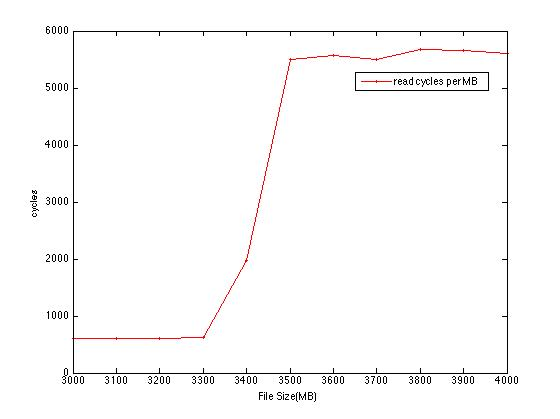
\includegraphics[width=5in]{./pics/41.jpg} 
   \caption{read cycles}
   \label{fig:read cycles}
\end{figure}

\paragraph{Discussion}
The graph shows that the file cache size is between 3300MB and 3500MB. Before this experiment, I did not realize that OS will use so many spaces for file cache. This optimisation speed up file reading time.